\documentclass{sig-alternate}

\usepackage{amsmath}
\usepackage{graphics}
\usepackage{graphicx}
\usepackage{subfigure}
\usepackage{color}
\usepackage{xspace}
\usepackage{url}
\usepackage[utf8]{inputenc}

% reviews
\newcommand{\todo}[1]        {\textcolor{red}{[TODO] #1}}
\newcommand{\keoma}[1]       {\textcolor{blue}{[Keoma] #1}}
\newcommand{\ana}[1]         {\textcolor{blue}{[Ana] #1}}
\newcommand{\diego}[1]       {\textcolor{blue}{[Diego] #1}}
\newcommand{\remy}[1]        {\textcolor{blue}{[Remy] #1}}
\newcommand{\xavi}[1]        {\textcolor{blue}{[Xavi] #1}}
\newcommand{\thomas}[1]      {\textcolor{blue}{[Thomas] #1}}

 % lorem
\newcommand{\lorem}          {\textcolor{green}{Lorem ipsum dolor sit amet, consectetur adipisicing elit, sed do eiusmod tempor incididunt ut labore et dolore magna aliqua. Ut enim ad minim veniam, quis nostrud exercitation ullamco laboris nisi ut aliquip ex ea commodo consequat. Duis aute irure dolor in reprehenderit in voluptate velit esse cillum dolore eu fugiat nulla pariatur. Excepteur sint occaecat cupidatat non proident, sunt in culpa qui officia deserunt mollit anim id est laborum.}}

% shortcuts
\newcommand{\smip}                {SmartMesh~IP\xspace}
\newcommand{\HRNEIGHBORS}         {{\tt HR\_NEIGHBORS}\xspace}
\newcommand{\HRDISCOVERED}        {{\tt HR\_DISCOVERED}\xspace}
\newcommand{\HRDEVICE}            {{\tt HR\_DEVICE}\xspace}
\newcommand{\pathcreate}          {{\tt path\_create}\xspace}
\newcommand{\pathdelete}          {{\tt path\_delete}\xspace}
\newcommand{\motecreate}          {{\tt mote\_create}\xspace}
\newcommand{\moteId}              {{\tt moteId}\xspace}
\newcommand{\NUMHRNEIGHBORS}      {140,897\xspace}

\graphicspath{{figures/}}

\begin{document}
\title{(Not so) Intuitive Results from a Smart Agriculture\\Low-Power Wireless Mesh Deployment}

\numberofauthors{6}
\author{
    \alignauthor Keoma~Brun-Laguna\\
        \affaddr{Inria, EVA team,\\ Paris, France}\\
        \email{keoma.brun@inria.fr}
    \alignauthor Ana~Laura~Diedrichs\\
        \affaddr{Universidad Tecnológica Nacional (UTN)\\Mendoza, Argentina}\\
        \email{ana.diedrichs@frm.utn.edu.ar}
    \alignauthor Diego~Dujovne\\
        \affaddr{Universidad Diego Portales}\\
        \affaddr{Santiago, Chile}\\
        \email{diego.dujovne@mail.udp.cl}
    \and
    \alignauthor R\'emy~L\'eone\\
        \affaddr{Inria, EVA team,\\ Paris, France}\\
        \email{remy.leone@inria.fr}
    \alignauthor Xavier~Vilajosana\\
        \affaddr{Univ. Oberta de Catalunya, Barcelona, Catalonia, Spain}\\
        \email{xvilajosana@uoc.edu}
    \alignauthor Thomas~Watteyne\\
        \affaddr{Inria, EVA team,\\ Paris, France}\\
        \email{thomas.watteyne@inria.fr}
}

\maketitle

\begin{abstract}
A 23-node low-power wireless mesh network is deployed in a peach orchard.
The network serves as a frost event prediction system.
On top of sensor values, devices also report network statistics.
In 4~months of operations, the network has produced over 2~million temperature values, and over 350,000~network statistics.
This paper presents an in-depth analysis of the statistics, in order to precisely understand the performance of the network.
Nodes in the network exhibit an expected lifetime between 4 and 16~years, with an end-to-end reliability of 100\%.
We show how -- contrary to popular belief -- wireless links are symmetric.
Thanks to the use of Time Slotted Channel Hopping (TSCH), the network topology is very stable, with $\leq$5 link changes per day in the entire network.
\end{abstract}

%==============================================================================
\section{Introduction}
\label{sec:intro}

% the problem

Peaches don't like frost.
If during the blooming season (September in Argentina), temperature gets below $-$3~C for only a couple of hours, the flowers freeze, and no peaches are produced.
In 2013, 85\% of the peach production in the Mendoza region (western Argentina) was lost because of frost events.
Farmers can lose everything in only a couple of hours.
Yet, if they are warned of a frost event a couple of hours ahead, they can install heaters throughout the orchards, and use big fans to move the hot air around.
Fighting the frost events is not the issue, what is hard is predicting it.

% the PEACH project

The goal of the PEACH project~\cite{watteyne16peach} is to predict frost events.
We install sensors around the orchard which measure air temperature, air relative humidity, soil moisture and soil temperature.
We feed the collected data into a database, and by analyzing the data in real-time using machine learning, we identify patterns in the data and predict frost events.

%======== front-page figure, do not move
\begin{figure}
    \centering
    \includegraphics[width=\columnwidth]{orchard}
    \caption{The wireless motes deployed in a peach orchard in Mendoza, Argentina.}
    \label{fig:orchard}
\end{figure}

% the architecture

Because of the heavy machinery which moves inside the orchard, using cables to interconnect the sensors is not an option.
Instead, we use \smip, an off-the-shelf low-power wireless mesh solution from Linear Technology.
The sensor devices are battery-powered and equipped with a radio.
They form a multi-hop topology, and collaborate to route the data generated by the devices (called ``motes'') to a gateway.
This gateway is connected to the Internet, and forwards the data gathered in the peach orchard in Argentina to the PEACH servers in Paris, France.
Data appears on the web interface on the servers seconds after it was gathered in the orchard.

\begin{figure*}
    \centering
    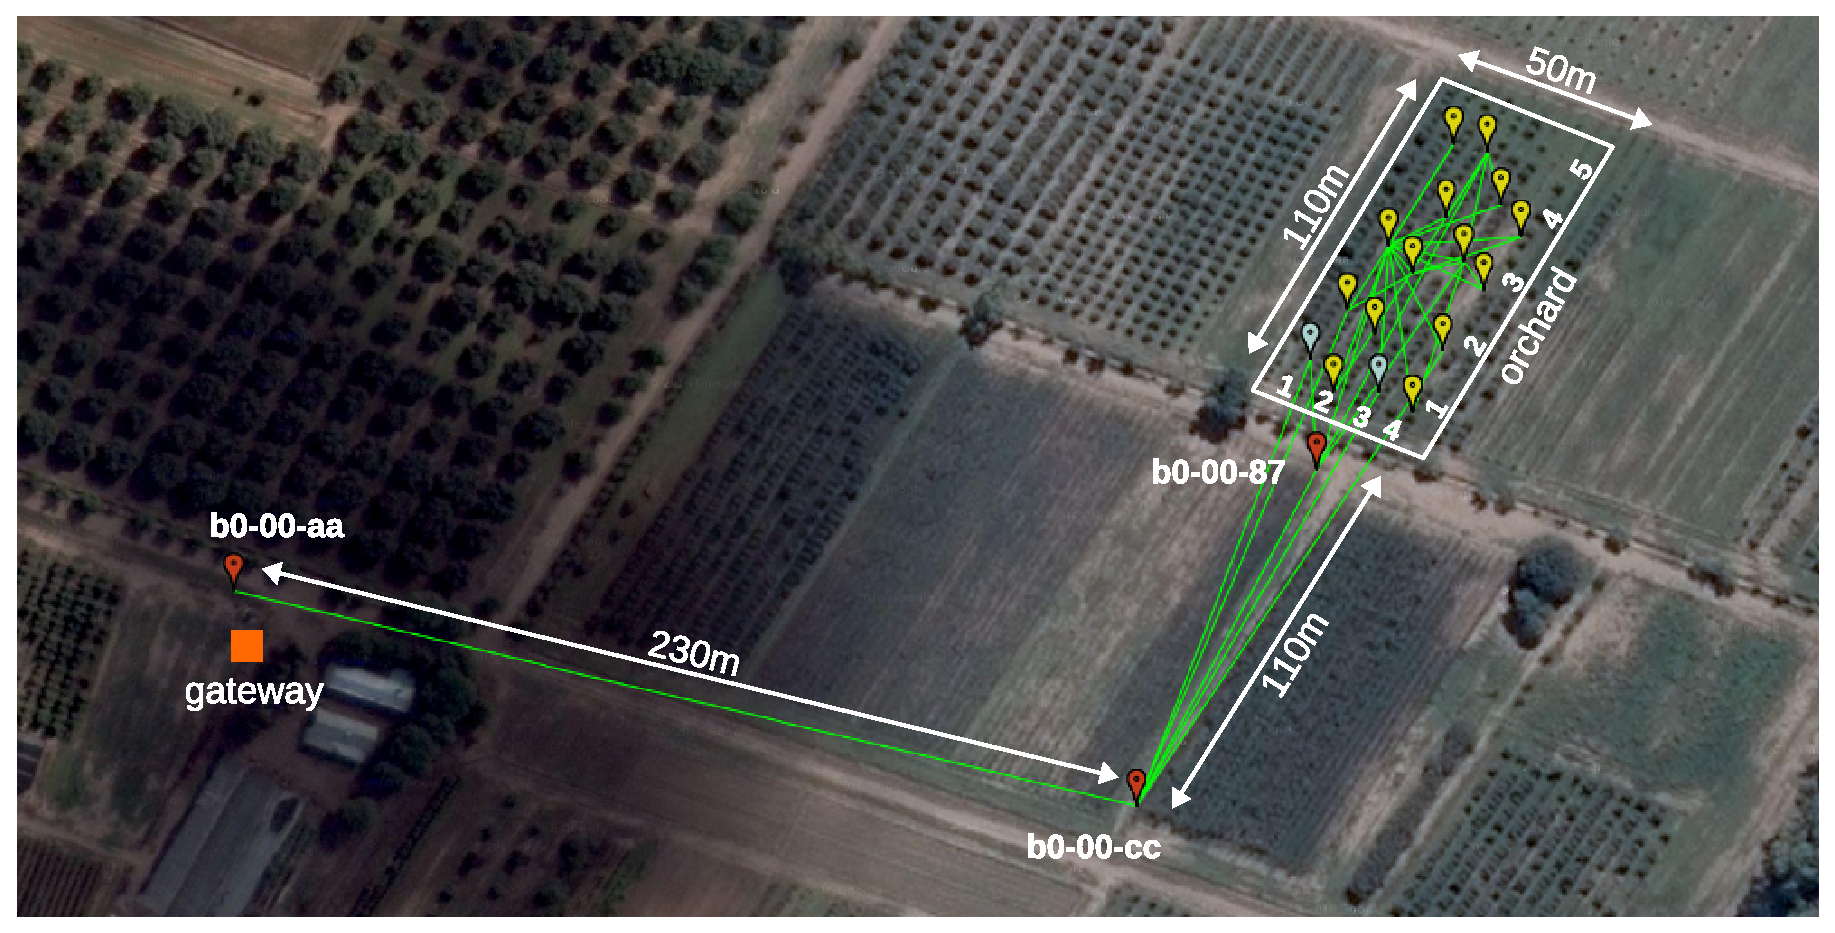
\includegraphics[width=\textwidth]{map_annotated}
    \caption{Areal view of the sensor network deployed in the orchard near Mendoza, Argentina.}
    \label{fig:map}
\end{figure*}

% the deployment

The network is deployed in a peach orchard of 204~trees, planted in a 50~m~$\times$~100~m area (shown in Fig.~\ref{fig:map}).
The low-power wireless network is composed of 18~sensor motes uniformly distributed between the peach trees, and 3~relay motes to connect the orchard to the gateway some 300~m away.
Each mote is placed in a water-tight box that is fixed on a 4~m high pole (see Fig.~\ref{fig:orchard}).

\begin{table}
\begin{center}
    \begin{tabular}{ | l | l | l | l | l |}
         \hline
         \tt{38-0f-66}     & \tt{60-05-78} &                   &               & 1 \\
         \tt{60-06-ec}     & \tt{60-05-ab} & \tt{60-02-4b}     & \tt{60-02-1b} & 2 \\
         \tt{60-05-5f}     & \tt{60-06-27} & \tt{60-05-69}     & \tt{60-01-f8} & 3 \\
         \tt{3f-fe-87}     & \tt{3f-fe-88} & \tt{60-06-0f}     & \tt{60-08-d5} & 4 \\
         \tt{30-60-ef}$^*$ & \tt{3f-f8-20} & \tt{58-32-36}$^*$ & \tt{60-03-82} & 5 \\
         \hline
           \multicolumn{1}{|c|}{1} & \multicolumn{1}{|c|}{2} & \multicolumn{1}{|c|}{3} & \multicolumn{1}{|c|}{4} &\\
         \hline
    \end{tabular}
    \caption{The MAC addresses of the motes inside the orchard (last 3 bytes). Refer to numbers displayed on the map. ($^*$) DC9018 node with external antenna.}
\end{center}
\end{table}

% hardware

We use four types of \smip devices.
The 2 DC9018 boards feature an external antenna; the 16 DC9003 boards a chip antenna.
These are deployed inside the orchard.
We deploy 3 long-range prototype boards outside the orchards to connect the orchard to the gateway.
The gateway is composed of a Raspberry~Pi single-board computer, and a DC2274 \smip manager.

% technology

The \smip network implements the IEEE802.15.4e standard~\cite{std_ieee802154e_2012}, which includes a channel hopping mechanism to reduce the impact of multipath fading and external interferences.
This allows the network to be highly reliable, stable, and extremely low power~\cite{watteyne10mitigating, watteyne09reliability}.

% the data

Each mote produces a temperature value every 30~s, and network statistics every 5~min.
In 4~months of operation, we gathered over than 2~million temperature values, and more than 350,000~network statistics.

% the goal of this paper

The goal of this paper is to analyze the network statistics over a 4~month period the network has been operating, and precisely assess the performance of the network.
This paper makes the following contributions:
\begin{itemize}
    \item We confirm that the \smip network exhibits years of battery lifetime and wire-like reliability;
    \item We show that channel hopping causes the network topology to be very stable, with $\leq$5 link changes per day;
    \item Contrary to popular belief, we show that links in the network are symmetric, i.e.~they exhibit the same signal strength in both directions of the same link.
\end{itemize}

% paper organisation

The remainder of this paper is organized as follows.
Section~\ref{sec:collected} describes what statistics we are collecting, and the amount of statistics collected over a 4~month period.
Section~\ref{sec:intuitive} presents results that confirm assumptions about what we can expect for real-world \smip deployment.
Section~\ref{sec:notsointuitive} presents not so intuitive results about link symmetry and network stability.
Finally, Section~\ref{sec:conclusion} concludes this paper and discusses further improvements.

%==============================================================================
\section{Statistics Collected}
\label{sec:collected}

% environment

The wireless network is deployed in a peach orchard in Junin, 45~km South-East of Mendoza in Western Argentina.
No other electronic devices are present in the field.
Farmers work inside the field with heavy machinery for 1-2~h every 20~days approximately.
In the region, air temperature ranges between $-$9~C in winter (May-October) to +38~C in summer (November-April).
Because of the sunny weather, day/night temperature swings of 20~C are not uncommon in winter.

% events and HR

Each device in the network produces both sensor data and network statistics.
Network statistics can be separated in Events and Health Reports messages.
\textit{Event} messages are non-periodic notifications the network sends when a network event happens (e.g.~a node joins/leaves the network, a link is created/deleted, etc.).
\textit{Health Report} (HR) messages are sent periodically by each mote; they contain counters and statistics about that mote.
HRs are used to assess the overall health of the network.

% number received and remainder

Table~\ref{tab:msg_stats} summarizes the number of events and HRs gathered during the 4~month period.
In the remainder of this section, we detail the meaning of each of the statistics.

\begin{table}
    \centering
    \begin{tabular}{|l|r|}
        \hline
        \multicolumn{1}{|c|}{type} & \multicolumn{1}{|c|}{number} \\ \hline
        \hline
        \motecreate     &     133         \\ \hline
        \pathcreate     &   4,098         \\ \hline
        \pathdelete     &   3,653         \\ \hline
        \HRDEVICE       & 132,758         \\ \hline
        \HRNEIGHBORS    & \NUMHRNEIGHBORS \\ \hline
        \HRDISCOVERED   &  87,737         \\ \hline
    \end{tabular}
    \caption{The number of statistics collected a 4~month period.}
    \label{tab:msg_stats}
\end{table}

% - - - - - - - - - - - - - -
\textbf{\motecreate.}
Each node in a \smip network can periodically send beacons to announce the presence of the network.
When a mote wants to join a network, it listens for those beacons.
Once it has heard a number of those, it starts a security handshake with the network.
During that handshake, the \smip manager send a \motecreate event notification over its serial port.
This is the event we log.
It contains, among other information, the association between the newly-joined device's 8-byte MAC address and its 2-byte \moteId.

% - - - - - - - - - - - - - -
\textbf{\pathcreate and \pathdelete.}
In \smip terminology, a ``path'' is the link-layer resource which allows two neighbor nodes to communicate\footnote{~In more classical networking terminology, this is often referred to as a ``link''. We use the terms ``path'' and ``link'' interchangeably in this paper.}.
Each time a mote starts communicating with a new neighbor (e.g.~its routing parent), a \pathcreate event is produced.
Similary, each time a mote \textit{stops} communicating with a neighbor (e.g.~it changes routing parent), a \pathdelete event is produced.
We log both messages.

% - - - - - - - - - - - - - -
\textbf{\HRDEVICE.}
Each network device produces a \HRDEVICE every 15~min.
This health report contains counters/statistics internal to the mote, such its current battery voltage, temperature, or total number of messages sent.

% - - - - - - - - - - - - - -
\textbf{\HRDISCOVERED.}
\smip nodes continuous monitor their surroundings to discover neighbor nodes.
Every 15~min, each node produces \HRDISCOVERED health report which contains the list of ``discovered'' neighbor, and the associate signal strength it heard it at.
These discovered neighbors can potentially be used in the future as neighbor the node communicates with.

% - - - - - - - - - - - - - -
\textbf{\HRNEIGHBORS.}
Two nodes are neighbors when they link-layer resources are installed for them to communicate.
The neighbors of a node are a subset of the discovered neighbors.
Every 15~min, each note generates a \HRNEIGHBORS health report which contains its list of neighbors.
These messages also specifies per-neighbor counters, such as the number of link-layer restransmissions.

% analysis

After 4~months of operation, we have collected 369,276~network statistics (see Table~\ref{tab:msg_stats}).
The goal of the next section is to present the main results from analyzing this information.
We group these results in two categories.
``Intuitive'' results (Section~\ref{sec:intuitive}) are results which confirm the performance expected from a \smip network.
``Not so intuitive'' results (Section~\ref{sec:notsointuitive}) are results which we believe go against popular belief.
This classification is necessarily subjective.

Possibly due to power line failure at the network manager side, the network experienced some restarting.
For this reason, some analysis presented in the next sections are done in shorter period.
As a side effect, this phenomenon allowed us to verify the network formation and joining process.

%==============================================================================
\section{Intuitive Results}
\label{sec:intuitive}

Previous publications~\cite{watteyne15industrial,watteyne16peach,watteyne10mitigating,watteyne09reliability} underlie the performance of TSCH networks in general, and \smip in particular.
Standardization work in the IETF 6TiSCH working group\footnote{~\url{https://tools.ietf.org/wg/6tisch/charters}} around TSCH networks further illustrate the move of the industrt towards this type networking technology.
So while we expect good performance from the network, this section verifies that this is indeed the case.
We start by looking at two physical-layer metrics: RSSI vs Distance (Section~\ref{sec:rssi_distance}) and PDR vs. RSSI (Section~\ref{sec:waterfall}).
While these have no dependency on TSCH (the type medium access), they allow us to verifyt the overall connectivity in the network.
We then look at key performance indicators of \smip networks: end-to-end reliability (Section~\ref{sec:net_reliability}) and network lifetime (Section~\ref{sec:lifetime}).

%------------------------------------------------------------------------------
\subsection{RSSI vs. Distance}
\label{sec:rssi_distance}

The Friis transmission model~\cite{saunders07antennas} gives the relationship between the Receive Signal Strength (RSSI)\footnote{~Strictly speaking, the RSSI is the Receive Signal Strength \textit{Indicator}, a value returned by radio chip. Because of its prevalence in low-power wireless literature, we use it RSS and RSSI interchangeably.} in free space.
While it does \textit{not} apply directly to our Smart Agriculture outdoor deployment, we node in Fig.~\ref{fig:pister_hack} that the individual RSSI values are located between the Friis model, and the Friis model offset by $-$40~dB.
This corroborates the results from~\cite{zats10wireless}.

\begin{figure}
    \centering
    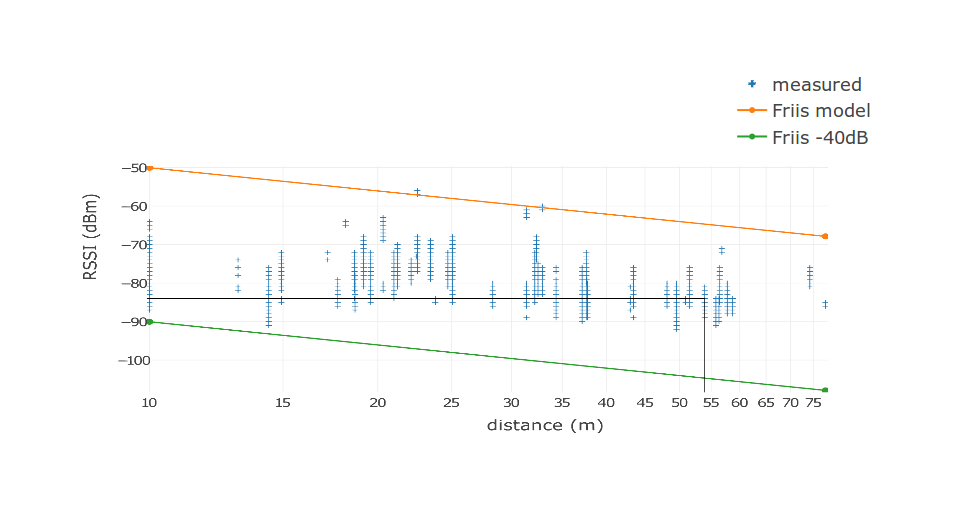
\includegraphics[width=\columnwidth]{pister_hack}
    \caption{RSSI measurements are roughly located between the Friis model and the Friis model shifted by $-$40~dB.}
    \label{fig:pister_hack}
\end{figure}

%------------------------------------------------------------------------------
\subsection{Wireless Waterfall}
\label{sec:waterfall}

% sample presentation

Due to the inherent physical unreliability of the radio medium, it is impossible to know if a future transmission will be successful or not.
The Packet Delivery Ratio (PDR) is the portion of successful link-layer transmissions over the total number of link-layer transmission attempts.
A failed attempt means that the link-layer frame needs to be re-transmitted; it does \textit{not} mean the packet is lost.
Over a period of 4~months, \NUMHRNEIGHBORS \HRNEIGHBORS messages are collected.
These contain, for a given node, the number of link-layer transmission attempts and successes to each of its neighbors.
We remove the portion of neighbors with no transmission (237,252 messages) and keep only the DC9003 motes, resulting in a total of 125,103 messages (approx. 27\% from the total number of \HRNEIGHBORS).

% plot

Fig.~\ref{fig:waterfall} plots the PDR and the RSSI of these 125,103 messages.
For readability, we also plot the average/deviation of the data for a given RSSI value.
Because of its shape, this is known as the ``waterfall plot''.

\begin{figure}
    \centering
    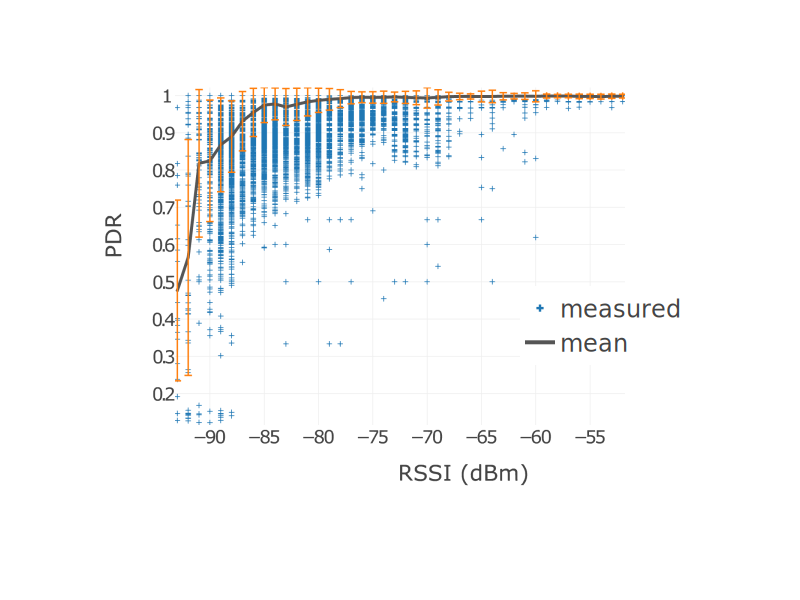
\includegraphics[width=\columnwidth]{waterfall}
    \caption{
        The PDR/RSSI waterfall.
        Links with low RSSI present good PDR showing the low interferences in the network.
    }
    \label{fig:waterfall}
\end{figure}

Overall, above $-$85~dBm, the PDR of the link is very good (>95\%).
Below that value, the PDR rapidly degrades, indicating that, on these links, frequent retransmissions will happen.
The device manufacturer documentation~\cite{smip_app_note} indicates that a path is considered as ``bad'' when:

\begin{itemize}
  \item RSSI>$-$80~dBm and PDR<50\%
  \item RSSI>$-$70~dBm and PDR<70\%
\end{itemize}

This is not the case here.

% interferences

A \textit{waterfall plot} either shifted right with very few paths below $-$70~dBm, or with non-constantly decreasing curve would be an example of interference-prone environment.
This is not the case if Fig.~\ref{fig:waterfall}, meaning that the \smip network is not suffering high levels of interferences from co-located wireless devices.

%------------------------------------------------------------------------------
\subsection{End-to-End Reliability}
\label{sec:net_reliability}

% steady state results

Table~\ref{tab:net_stats} presents the statistics from the last time the network restarted (i.e 10 days).
The results correspond to the ones presented in the project presentation paper~\cite{watteyne16peach} as stated:
``After approx. 24~hours of operation, a \smip network reaches steady state''.

All the 693,844 messages produced by the sensor network were received by the network gateway.
The stability, i.e the average PDR over the different links, increased of 2\%.
The latency, i.e the averaged time a message travel inside the network, lowered from 700~ms to 800~ms.

\begin{table}
    \begin{tabular}{|l|l|}
        \hline
        reliability & 100\% (Arrived/Lost:   693844/0)\\ \hline
        stability   & 95\% (Transmit/Fails: 4405569/258778)\\ \hline
        latency     & 700~msec\\
        \hline
    \end{tabular}
    \caption{The overall network statistic over the last 10 days.}
    \label{tab:net_stats}
\end{table}

%------------------------------------------------------------------------------
\subsection{Network Lifetime}
\label{sec:lifetime}

% description

Each device is powered by a pair of AA battery (Energizer L-91) with a charge of approximately 2821mAh.
The charge is measured by a built-in sensor inside the \smip board. \keoma{@thomas: could you give me more details?}

% results

Fig.\ref{tab:stats_charge} shows the device charge statistics over a 4-month period.
Every node is crucial in this application as each mode is connected to multiple sensors and represents one part of the orchard that could be prone to frost.
We thus consider the network lifetime as the time when the first node runs out of battery.
The node with the maximal amount of days left is node {\tt 60-02-4b}.
From~Fig.\ref{fig:map}, we can see that the node has no child and thus, do not retransmit any data from its neighbors.
The node with the minimal lifetime is node {\tt b0-00-cc} , that is one of the long-range node that is used to link up the orchard motes to the network gateway, see Fig.\ref{fig:map}.
It is normal that this node spend more energy than the others as all the traffic passes through it.
While being the most loaded node, {\tt b0-00-cc} has above 4 years lifetime.
This shows the very low consumption of the wireless mesh network.

\keoma{the same node had a 5.18 years lifetime in prev paper, should we explain it ?}

\begin{table}
  \begin{tabular}{|c|c|r|}
     \hline
     MAC address    & charge consumed           &   lifetime \\
     \hline
     \tt{30-60-ef}  & 227,847~C (2.2\% battery) & 10.8~years \\
     \tt{38-0f-66}  & 252,356~C (2.5\% battery) &  9.8~years \\
     \tt{3f-f8-20}  & 291,312~C (2.9\% battery) &  8.4~years \\
     \tt{3f-fe-87}  & 392,606~C (3.9\% battery) &  6.3~years \\
     \tt{3f-fe-88}  & 458,459~C (4.5\% battery) &  5.3~years \\
     \tt{58-32-36}  & 327,634~C (3.2\% battery) &  7.5~years \\
     \tt{60-01-f8}  & 252,454~C (2.5\% battery) &  9.8~years \\
     \tt{60-02-1b}  & 222,253~C (2.2\% battery) & 10.1~years \\
     \tt{60-02-4b}  & 146,068~C (1.4\% battery) & 16.8~years \\
     \tt{60-03-82}  & 494,841~C (4.9\% battery) &  5.0~years \\
     \tt{60-05-5f}  & 274,502~C (2.7\% battery) &  9.0~years \\
     \tt{60-05-69}  & 437,136~C (4.3\% battery) &  5.7~years \\
     \tt{60-05-78}  & 304,145~C (3.0\% battery) &  8.1~years \\
     \tt{60-05-ab}  & 284,764~C (2.8\% battery) &  8.7~years \\
     \tt{60-06-27}  & 321,879~C (3.2\% battery) &  7.7~years \\
     \tt{60-08-d5}  & 263,120~C (2.6\% battery) &  9.3~years \\
     \tt{b0-00-87}  & 199,626~C (2.0\% battery) & 12.3~years \\
     \tt{b0-00-aa}  & 544,439~C (5.4\% battery) &  4.5~years \\
     \tt{b0-00-cc}  & 567,232~C (5.6\% battery) &  4.3~years \\
     \hline
  \end{tabular}
  \caption{The charge statistics.}
  \label{tab:stats_charge}
\end{table}

%==============================================================================
\section{Not so Intuitive Results}
\label{sec:notsointuitive}

After presenting the intuitive results, this section shows results that are not straightforward.
We first show that assuming link asymmetry is not always true by presenting very symmetrical RSSI values when using the same devices an multiple frequencies.
We then show the high network stability a TSCH-based network can provide by looking at the path creation and deletion over days.

%------------------------------------------------------------------------------
\subsection{Link (A)Symmetry}
\label{sec:symmetry}

% RSSI expectations

The RSSI values can be retrieved from both active neighbors and discovered neighbors Health Reports, thus every 15~min for each pair of device.
Those RSSI values are averaged values over the 16 channels defined in the IEEE 802.15.4 standard~\cite{std_ieee802154_2011}.
In the rest of that paper we will use RSSI to denote the average RSSI over the 16 channels.

% environment

The peach orchard is located in a rural area that is not exposed to high traffic on the ISM band so we do not expect important external interferences.
Heavy machinery is used inside the orchard by farmers approximately every 20 days and during a period of one to two hours.
Those movements could create internal interferences such as multipath fading.

% symmetry analysis

A common assumption is to assume that a layer 2 link between two identical wireless nodes is asymmetrical.
We looked at the link statistics between the 18th of June and the 4th of July (16 days) and analysed the difference between the RSSI values.
The sample contains 411132 \HRNEIGHBORS messages and concerns 14 nodes with the same hardware (DC9003).
During that period, 21 different bidirectional links are active with at least 250 transmissions for each link.
For each of those links, we compute the RSSI difference between the two directions of the link (i.e from A to B and from B to A) and present the results in Fig.~\ref{fig:tab_symmetry}).
The very low RSSI difference shows that the links are very symmetrical.
Note that the RSSI is an averaged value over the different channels.

\begin{figure}
    \centering
    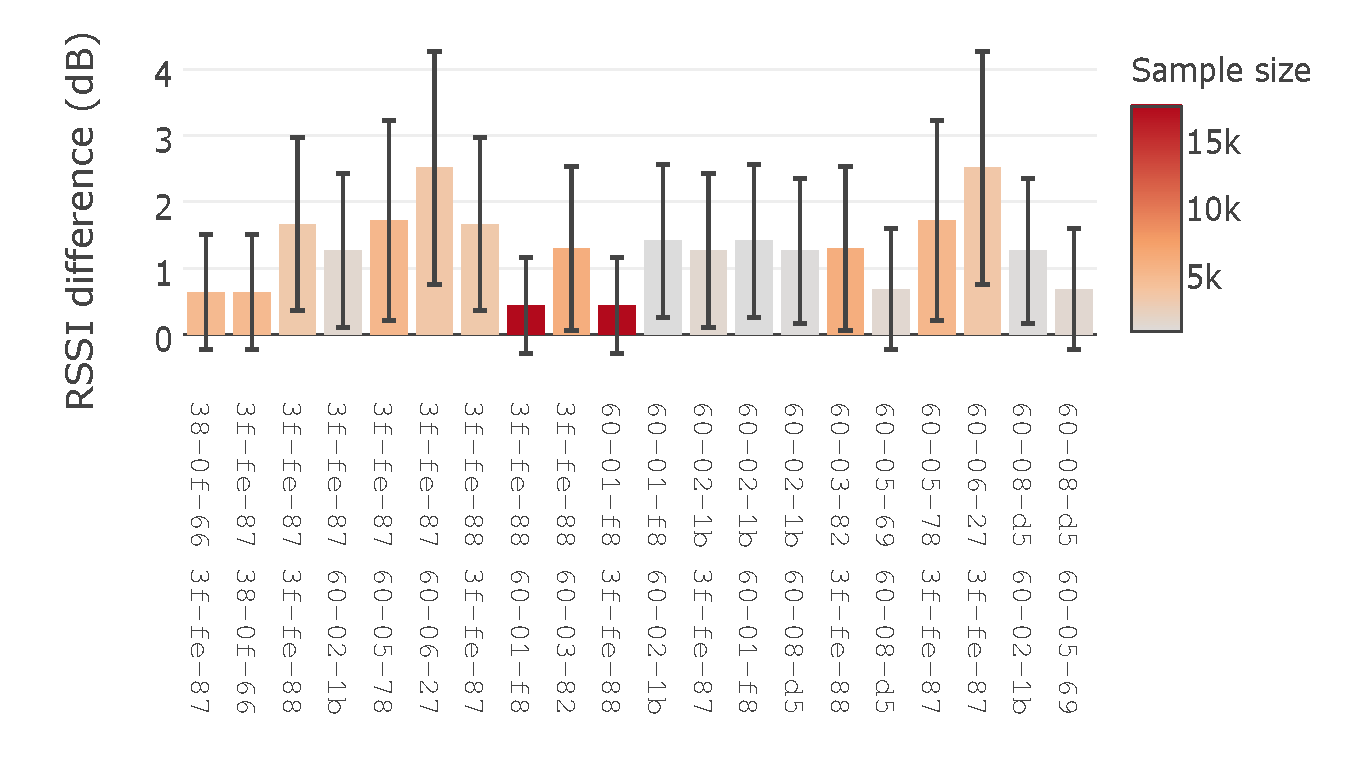
\includegraphics[width=\columnwidth]{sym_plot}
    \caption{The different active links between 2016-06-18 and 2016-06-25.}
    \label{fig:tab_symmetry}
\end{figure}

%------------------------------------------------------------------------------
\subsection{Network Stability}
\label{sec:net_stability}

% description

The nodes in the network form a Destination Oriented Direct Acyclic Graph (DODAG) oriented toward the gateway (i.e the DAG root).
Each node maintains a list of neighbors, with which they communicate or not, and dynamically change their routes depending on link quality. \keoma{@thomas:is it true ? or they use other metrics ?}
When reliability is high the network topology stay stable and the nodes use the same neighbors.
When the reliability decreases on a certain path, nodes select other neighbors, making the network topology to change.
Instability in the network increases the signaling traffic to reconstruct the routes and introduce more bandwidth and energy consumption.

% dataset

To study the network stability we use the \pathdelete and \pathcreate event messages described in Section~\ref{sec:collected}.
Those messages are sent every time a path with a neighbor is deleted or created responsively.
Node {\tt b0-00-cc} was removed from the dataset as it does not respect the Dust requirement of having at least two parents to associate with.
Due to the lack of second parent the node was producing more than 20 time amount of messages than all the other nodes assembled.

% results

Fig.\ref{fig:net_churn} shows the number of events message per hour as well as the total number of links per hour over a two-weeks period.
We can see that the number of links stay close to 35 for the entire period.
The number of \pathcreate and \pathdelete is also kept low.

\begin{figure}
    \centering
    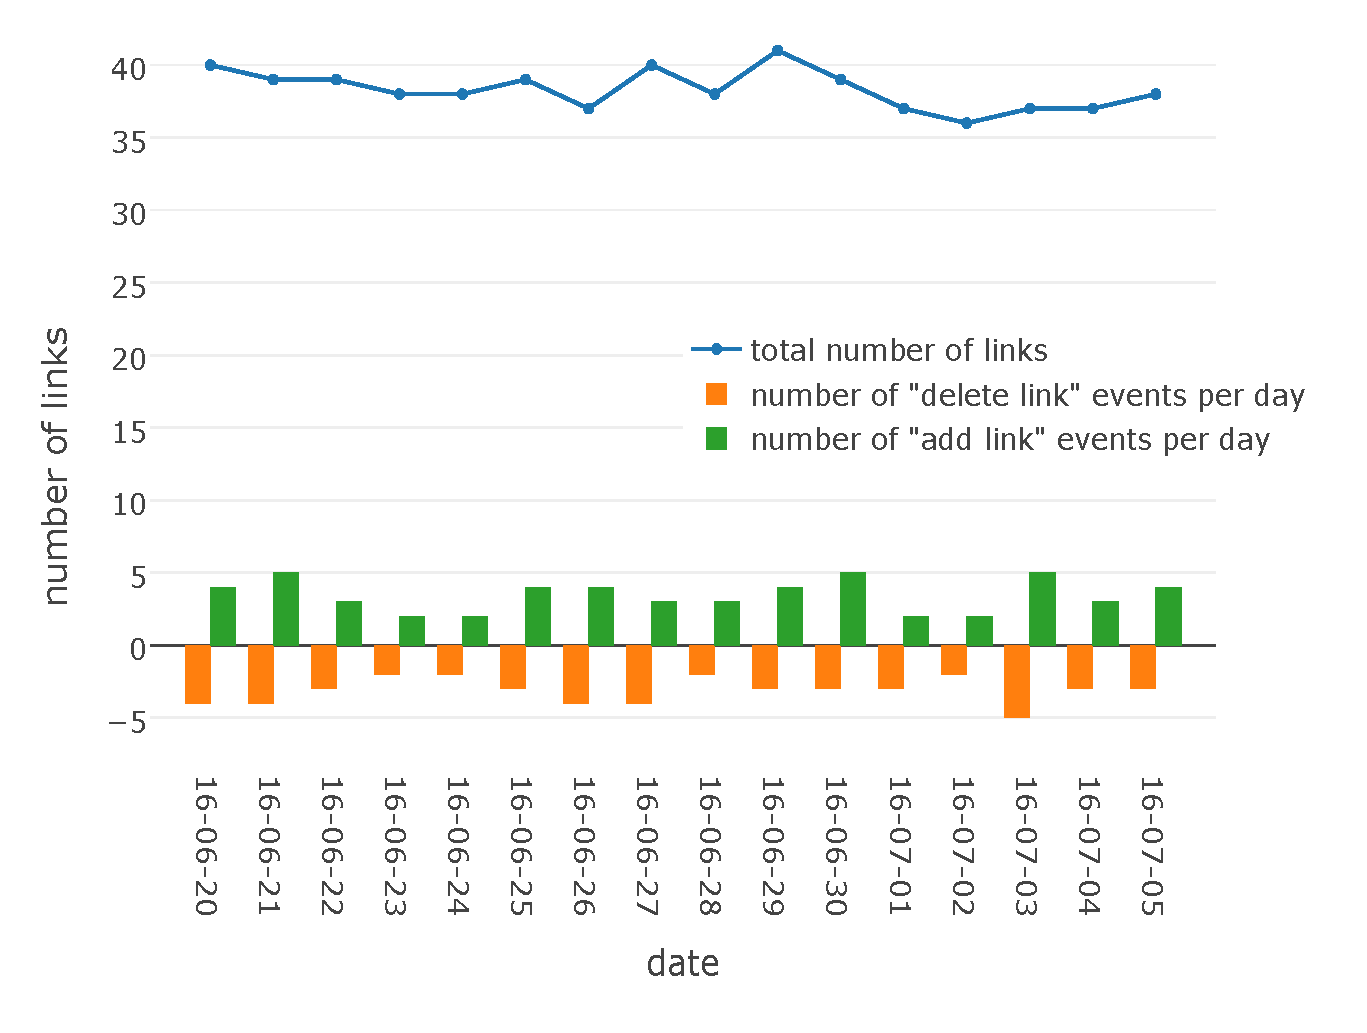
\includegraphics[width=\columnwidth]{net_churn}
    \caption{Network churn.}
    \label{fig:net_churn}
\end{figure}

%==============================================================================
\section{Conclusion}
\label{sec:conclusion}

The PEACH project started in April 2016 to build a low-power wireless sensor network based, turn-key solution to predict frost event in peach orchards.
After 4 months of measurements, we present the first data analysis from the collected data.\\

Some results are intuitive.\\
1. The RSSI against distance measurements follow the Friis transmission equation.
2. The relation between RSSI and PDR shows that interferences inside the field are low.
3. The overall network statistics that are reliability, stability and latency did not change much compared to the project first 24~hours measurements.
This shows that the network statistics are highly predictable.\\
4. The nodes that relay more traffic spend more energy than the other nodes.
The most loaded note has a 4.3~years lifetime showing the extremely low consumption of the network.\\

Some results are not intuitive.\\
1. While it is often assumed that RSSI is asymmetrical between two nodes, we show that when considering the averaged RSSI over the 16 different IEEE802.15.4 channels, links are very symmetrical.
2. The TSCH based network can show very high stability.
We observed less than 5 path modifications per hour during a two weeks period.\\

This first study prepares the ground for the next stage of the project where we will add additional sensors and present frost prediction results.


%==============================================================================

\bibliographystyle{abbrv}
\bibliography{brun16intuitive}

\end{document}
